\documentclass[11pt]{article}
\usepackage[top=1.00in, bottom=1.0in, left=1.1in, right=1.1in]{geometry}
\renewcommand{\baselinestretch}{1}
\usepackage{graphicx}
\usepackage{natbib}
\usepackage{amsmath}
\usepackage{hyperref}
\usepackage{todonotes}


\def\labelitemi{--}
\parindent=0pt
\parskip=5pt

\begin{document}
\bibliographystyle{/Users/Lizzie/Documents/EndnoteRelated/Bibtex/styles/besjournals}

\title{Effects of phenology on plant community assembly and structure }
\author{}
\date{\today}
\maketitle
\tableofcontents

Phenology definitions ...\\
the timing of critical stages of growth/reproduction and the transitions between them\\
timing of recurring growth and reproductive events (Ackerly)\\


% Need ref for Janneke 2012 review (HilleRisLambers et al.)
Communities assemble from a regional species pool through a series of abiotic and biotic sorting processes. At the largest scale, a community's species assemblage is limited by species in the larger regional pool---species well suited to an environment may thus not appear in it unless they are present in the this regional pool. From this pool, species are filtered based on the abiotic environmental conditions of a particular location---species must be able to persist through an environments extremes in hot, cold, dry, wet and other factors to pass through this `environmental filtering' step of assembly. This collection of potential species that could form a community is then filtered once more---by the pool of species itself. Competitive, facilitative, predatory and all other biotic interactions will determine which species together can co-occur in the long term. If two species compete too strongly, then only the stronger competitor will remain in the community at this step, and similarly obligate mutualists, predators and parasites will persist only if the other species they require are present in the community. % TO DO: Should I say coexistence here? Yes! And acknowledge there are competing theories for it. 

Species phenology is critical to both the environmental and biotic filtering steps of community assembly. % TO DO: Is this a tag-on to end of last paragraph (and tweak topic sentence) or is it a full paragraph?

\section*{}


\bibliography{/Users/Lizzie/Documents/git/bibtex/LizzieMainMinimal.bib}

\section{Figures}
\begin{figure}[h!]
\centering
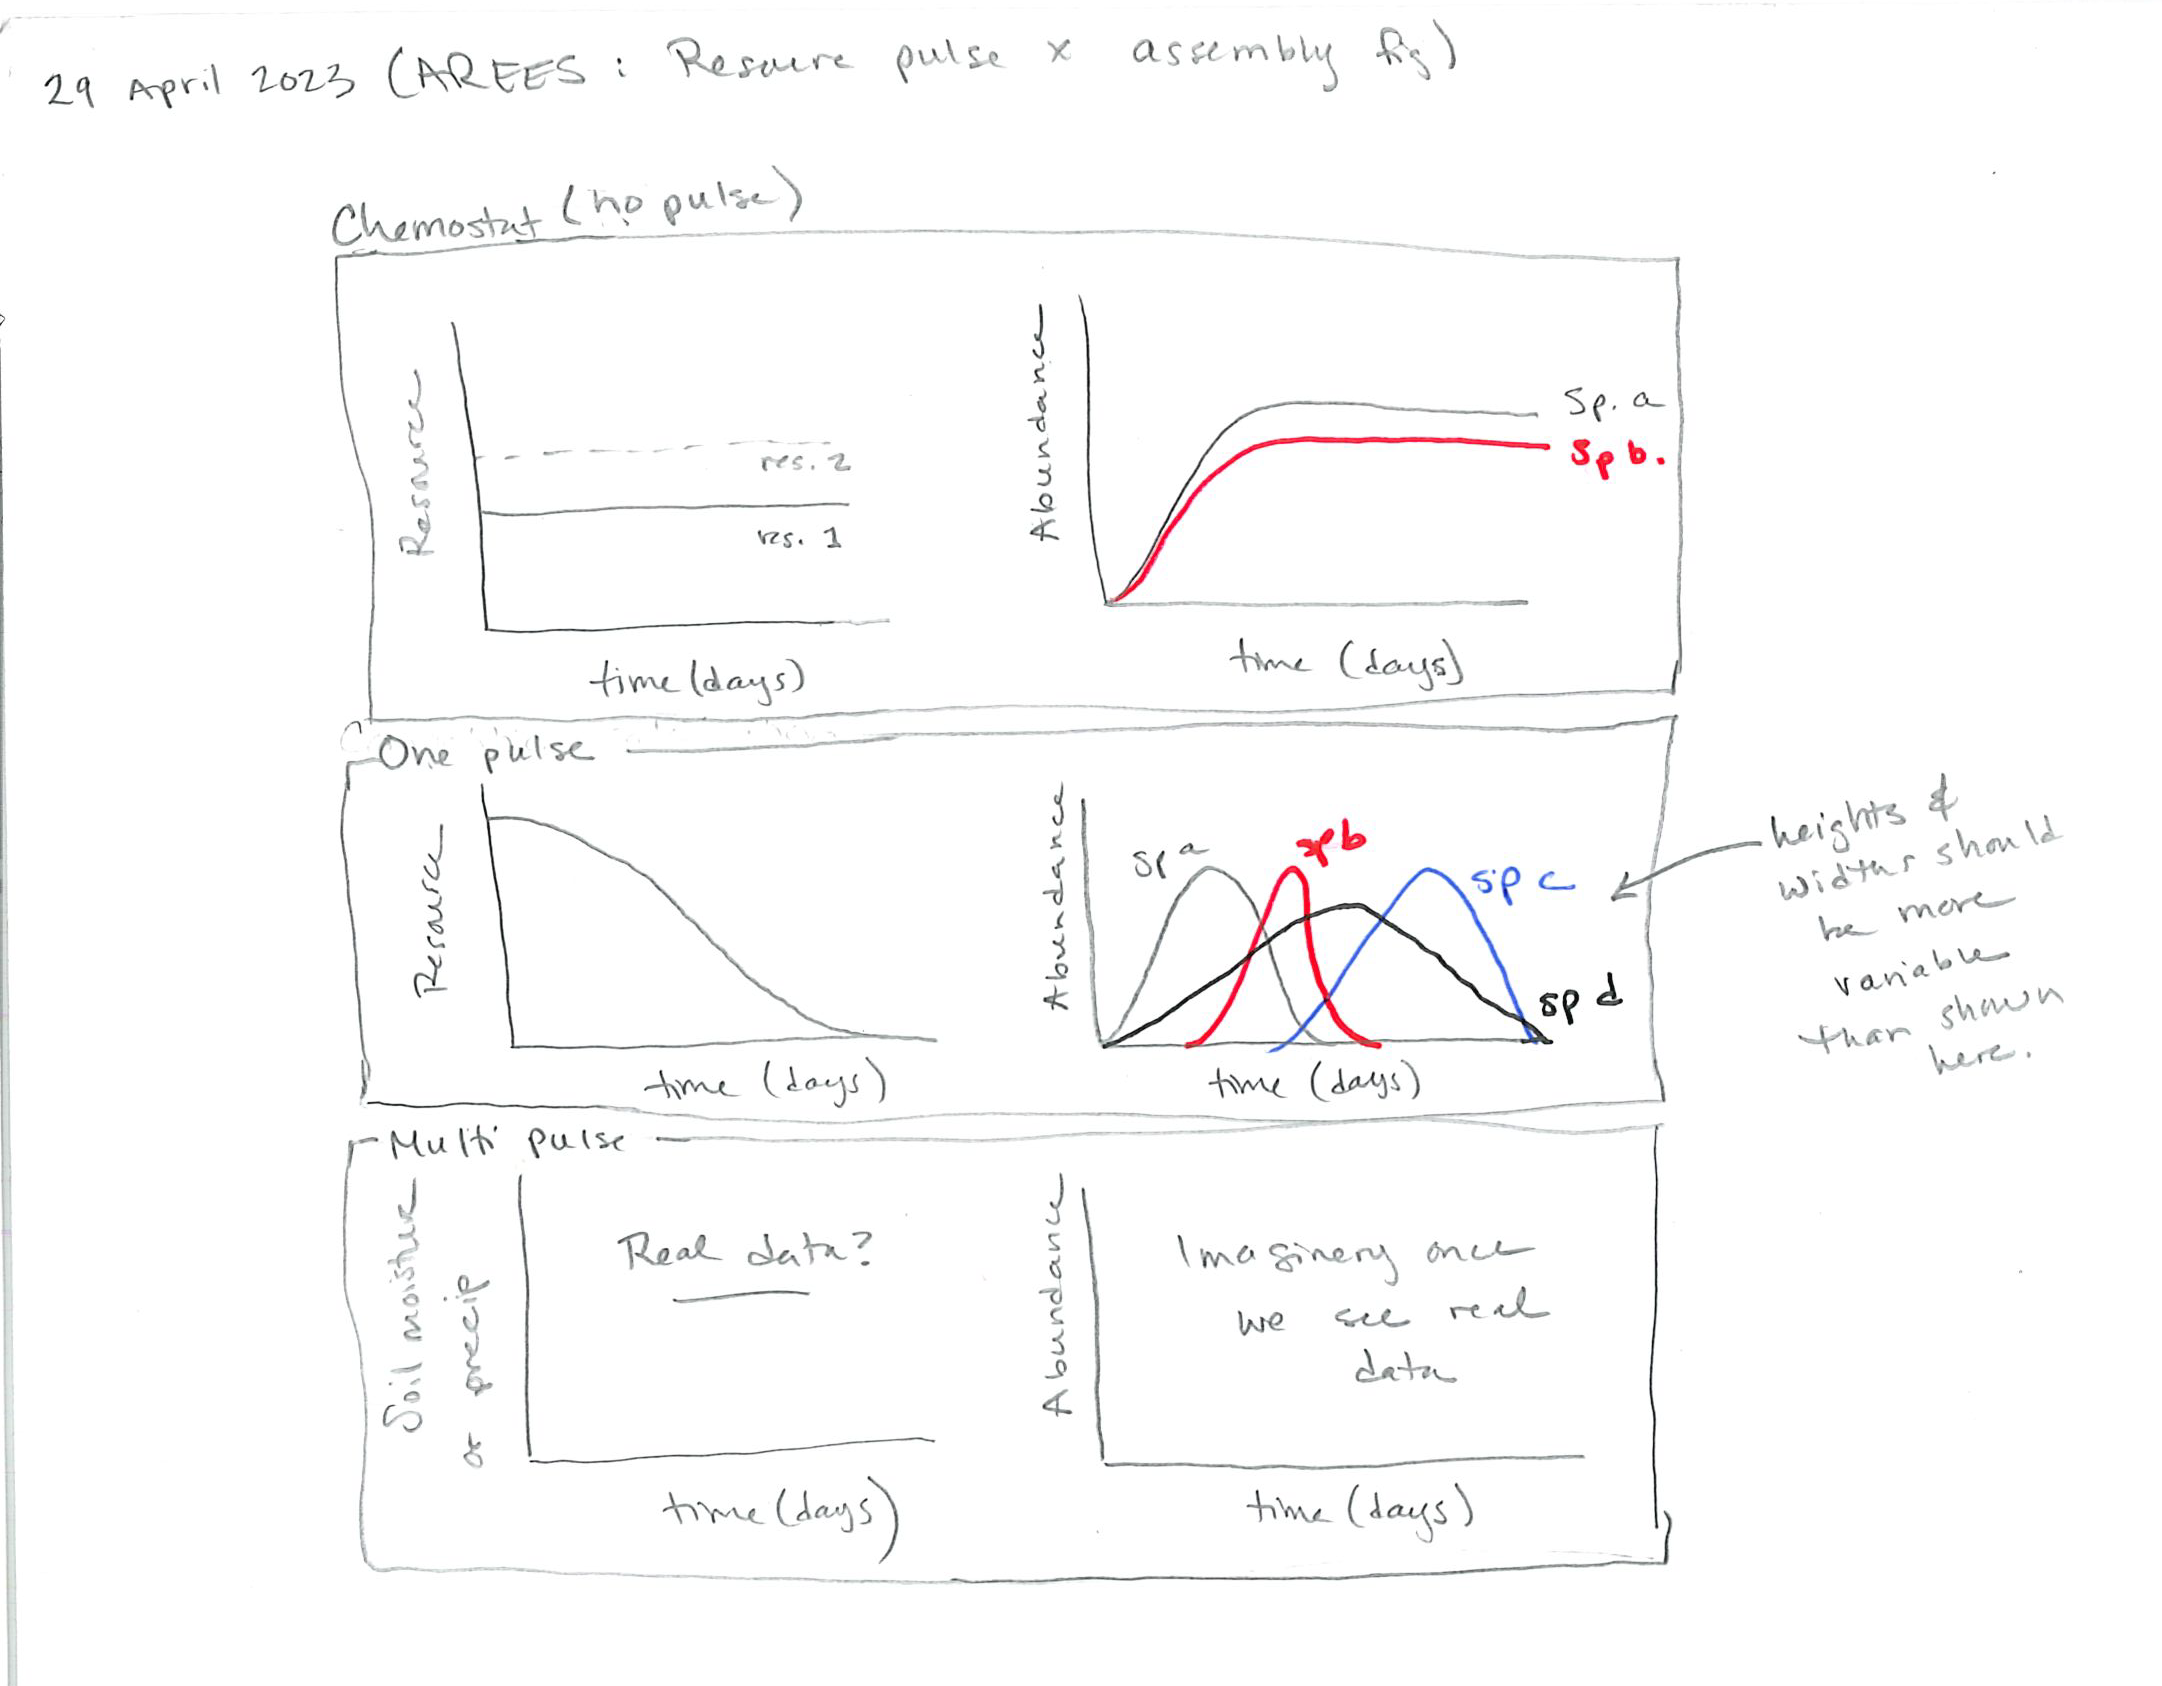
\includegraphics[width=1\textwidth]{..//figures/FigResourceApr2023.png}
\caption{Theory suggests resource levels may determine temporal niche space. In a system where resources are constant (top left,, chemostat; species can only coexist if they are each equally good competitors for different resources) species would be expected to show little temporal fluctuations. Many models of coexistence today, however, assume a resource pulse that decays (middle, left; e.g., water with evaporative loss) over time: this resource then sets the temporal window of each season and species compete within it. Most real systems however are more complicated (bottom left) ....}
 \label{fig:resource}
\end{figure}



\end{document}
